\documentclass[10pt, twocolumn]{article}

\usepackage[margin=0.75in]{geometry}
\usepackage{amsmath,amsthm,amssymb}
\usepackage{xcolor}
\usepackage{cancel}
\usepackage{graphicx}
\usepackage{changepage}
\usepackage{lipsum}
\usepackage{circuitikz}
\usepackage{pgfplots}
\usepackage{physics}
\usepackage{hyperref}
\usepackage{siunitx}
\usepackage{fontspec}
\usepackage{tikzsymbols}
\usepackage{subfig}
\usepackage{cuted}
\usepackage{multicol, multirow, booktabs}
\usepackage[breakable]{tcolorbox}
\usepackage[inline]{enumitem}

\theoremstyle{definition}
\newtheorem{problem}{Problem}
\newtheorem{soln}{Solution}

\pgfplotsset{compat=newest}
\usetikzlibrary{lindenmayersystems}
\usetikzlibrary{arrows}
\usetikzlibrary{calc}

\definecolor{incolor}{HTML}{303F9F}
\definecolor{outcolor}{HTML}{D84315}
\definecolor{cellborder}{HTML}{CFCFCF}
\definecolor{cellbackground}{HTML}{F7F7F7}
\newcommand{\ui}{\hat{i}}
\newcommand{\uj}{\hat{j}}
\newcommand{\uk}{\hat{k}}
\newcommand{\ux}{\hat{x}}
\newcommand{\uy}{\hat{y}}
\newcommand{\uz}{\hat{z}}
\newcommand{\primed}[1]{#1^\prime}
\usetikzlibrary{positioning, fit, calc}
\pgfdeclarelayer{background}  
\pgfsetlayers{background,main}
\AtBeginDocument{\RenewCommandCopy\qty\SI}

\makeatletter
\newcommand{\boxspacing}{\kern\kvtcb@left@rule\kern\kvtcb@boxsep}
\makeatother
\newcommand{\prompt}[4]{
    \ttfamily\llap{{\color{#2}[#3]:\hspace{3pt}#4}}\vspace{-\baselineskip}
}

\newcommand{\thevenin}[2]{
  \begin{center}
    \begin{circuitikz} \draw
      (0,0) -- (2,0) to[battery1, l_=$V_{Th}\eq#1$] (2,2) 
      to[resistor, l_=$R_{Th}\eq#2$] (0,2)
      ;
      \draw [o-] (-.07,2.079);
      \draw [o-] (-.07,0.079);
    \end{circuitikz}
  \end{center}
}

\newcommand{\norton}[2]{
  \begin{center}
    \begin{circuitikz} \draw
      (0,0) -- (3,0) to[american current source, l_=$I_{N}\eq#1$] (3,2) -- (0,2) (2,0)
      to[resistor, l=$R_{N}\eq#2$] (2,2)
      ;
      \draw [o-] (-.07,2.079);
      \draw [o-] (-.07,0.079);
    \end{circuitikz}
  \end{center}
}

\newcommand{\highlight}[1]{\colorbox{yellow}{$\displaystyle #1$}}

\newcommand{\ti}[1]{\widetilde{#1}}

\newfontface{\Kaufmann}{Kaufmann}
\DeclareTextFontCommand{\kf}{\Kaufmann}
\newcommand{\scriptr}{\fontsize{12pt}{12pt}\kf{r}}

\newfontface{\KaufmannB}{Kaufmann Bd BT}
\DeclareTextFontCommand{\kfb}{\KaufmannB}
\newcommand{\bscriptr}{\fontsize{12pt}{12pt}\kfb{r}}

\newcommand{\bv}[1]{\mathbf{#1}}

\title{Physics 3200Y: Prelab 1 - Lorem Ipsum, a Story}
\author{Jeremy Favro (0805980) \\ Trent University, Peterborough, ON, Canada}
\date{\today}

\begin{document}
\maketitle
\section{Lorem}
\lipsum[1]
\subsection{Ipsum}
\lipsum[2]
\subsection{Dolor sit}
\lipsum[3]
\subsection{Amet}
\lipsum[5]
\section{An Equation}
$$
    F=\sum_{i=1}^{n}F_n=\frac{1}{4\pi\epsilon_0}\sum_{i=0}^{n}\frac{q_iQ}{\scriptr_i^2}\hat{\bscriptr_i}=\frac{Q}{4\pi\epsilon_0}\sum_{i=0}^{n}\frac{q_i}{\scriptr_i^2}\hat{\bscriptr_i}
$$
Where $F$ is the net force on $Q$ due to charges $q_1,\dots,q_n$ each at distances $\scriptr_1,\dots\scriptr_n$ where $\scriptr$ is AN ACTUAL CHARACTER INSTEAD OF A PDF which means I can
\begin{strip}
    \begin{center}
        \foreach \n in {10,...,50}{\fontsize{\n pt}{\n pt}\kfb{r}}
    \end{center}
\end{strip}
without raster effects which is nice \Laughey[1.4].
\newpage ~
\section{My Cats}
\begin{figure}[ht!]
    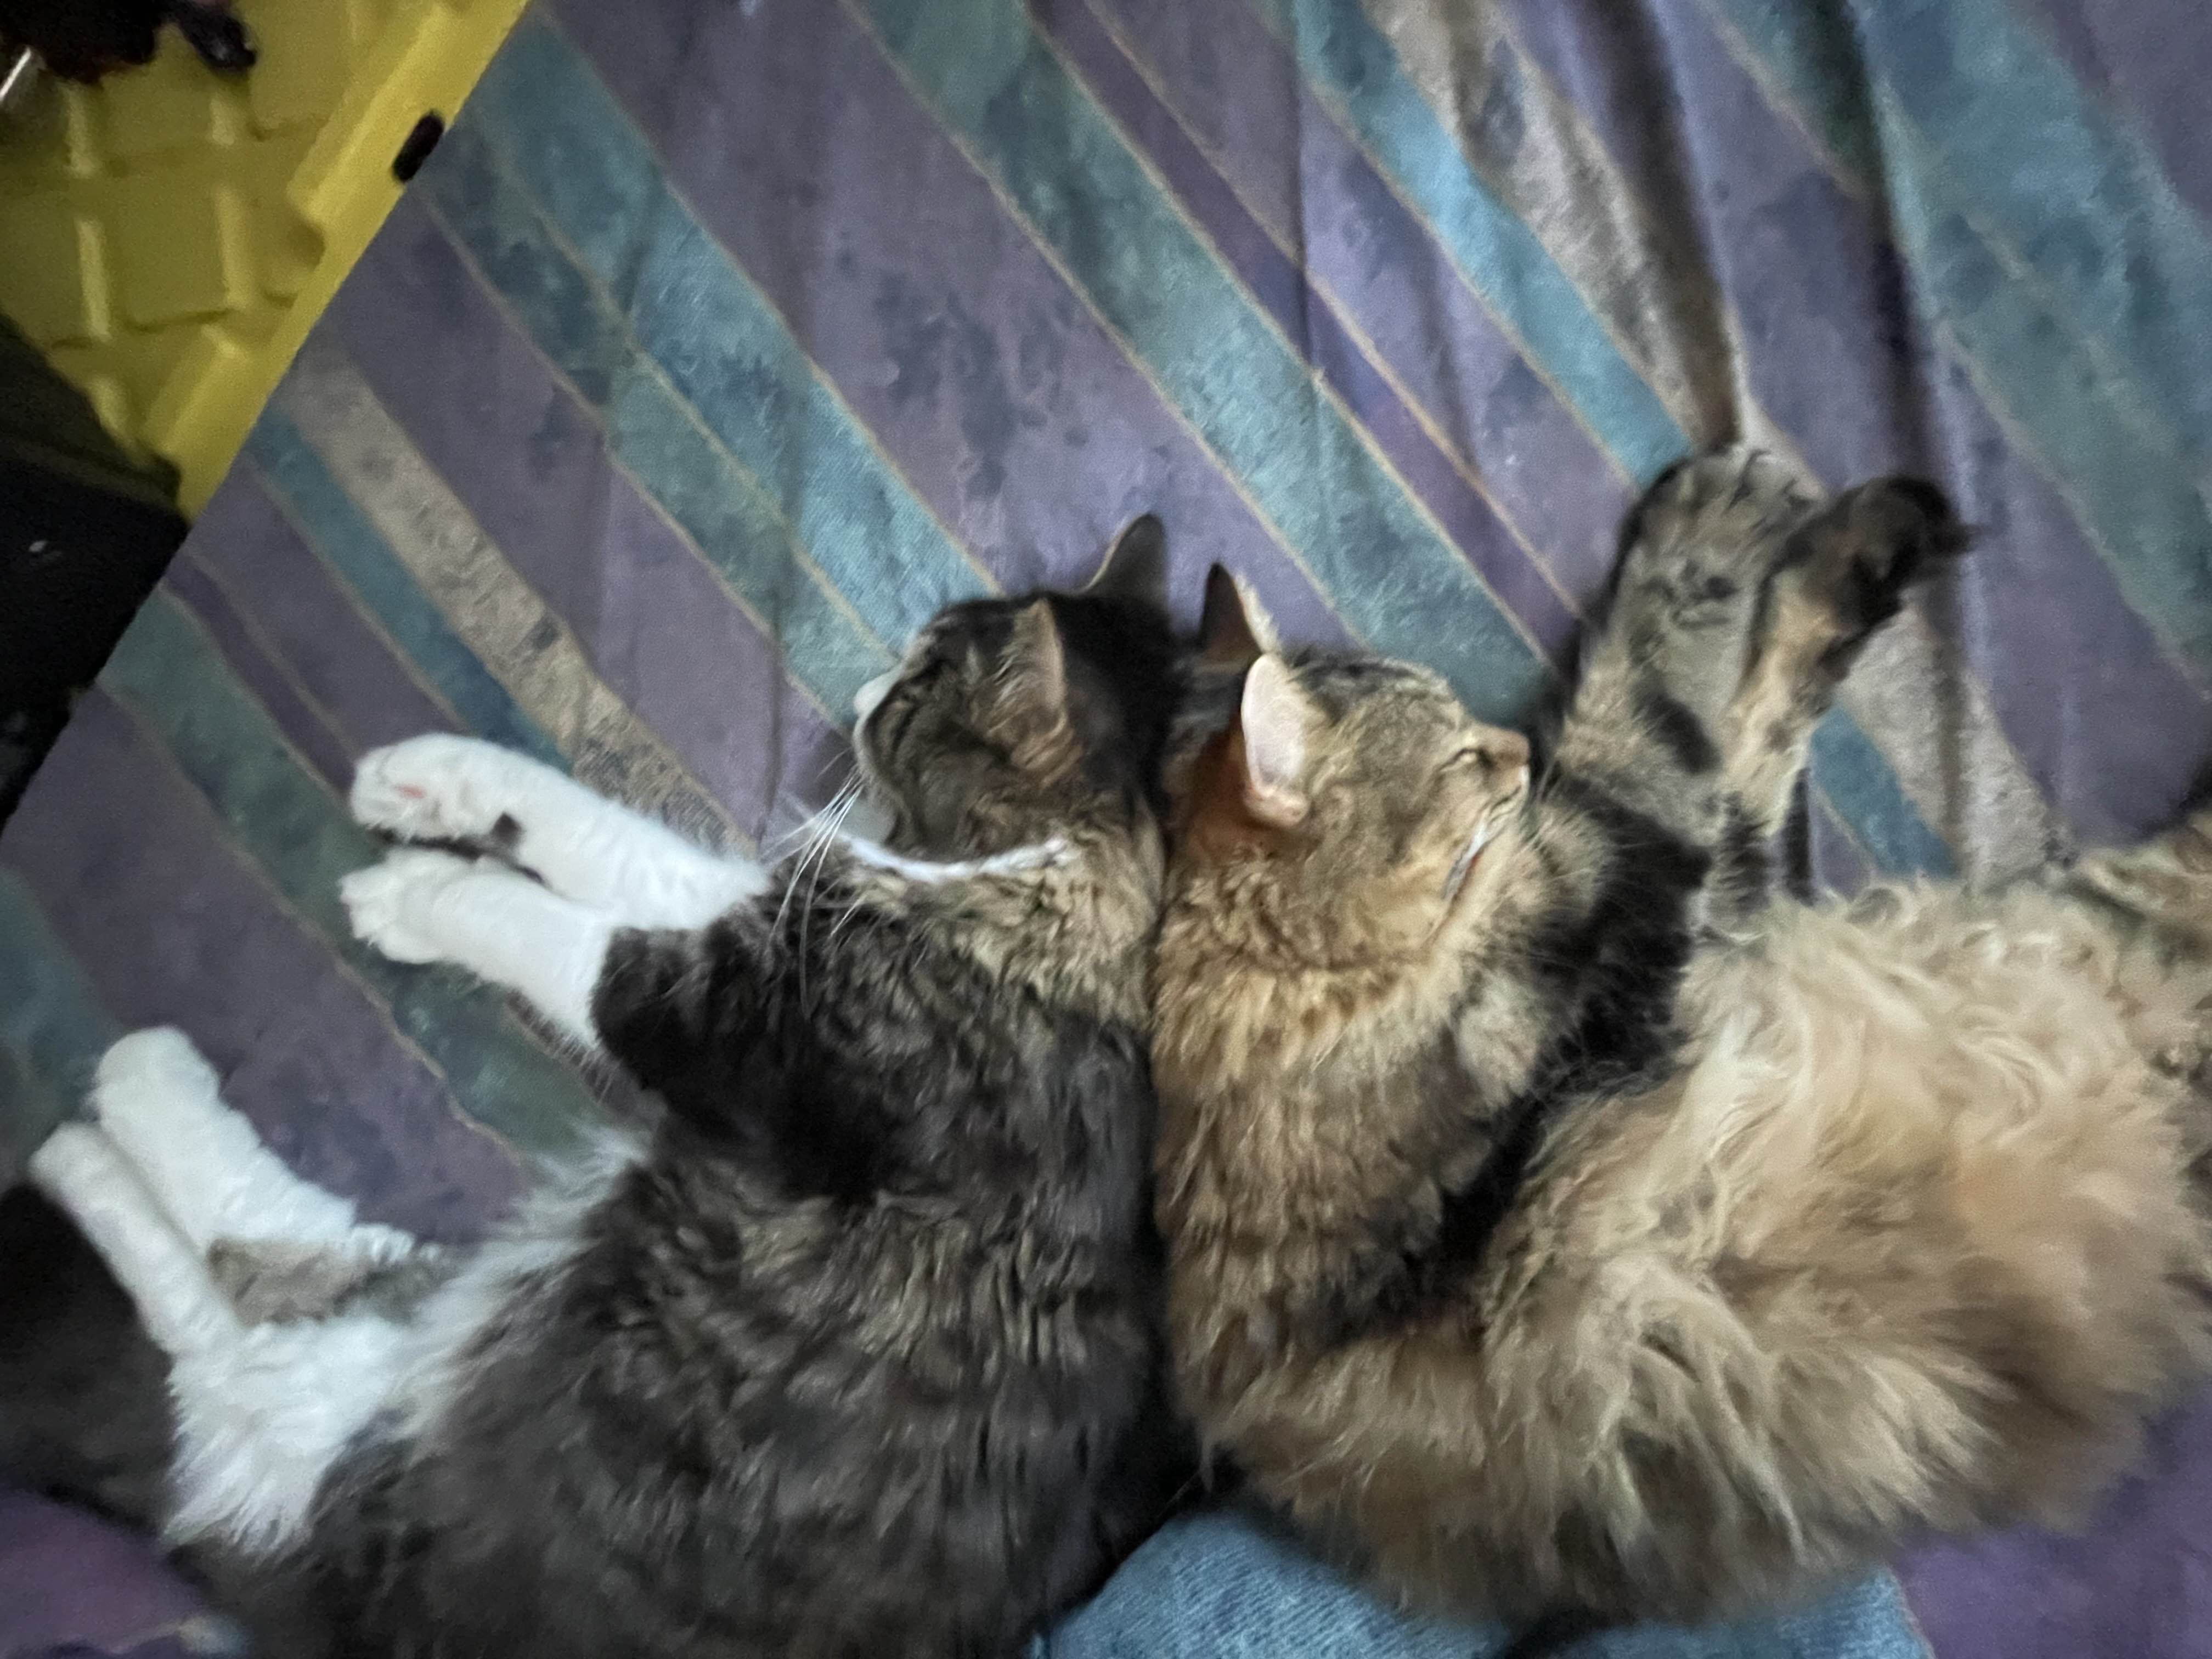
\includegraphics[scale=0.05]{cats.png}
    \centering
    \caption{My cats \Cat[1.4] \Laughey[1.4]}
\end{figure}
\section{Important Data}
\begin{table}[h]
    \centering%
    \caption{Observed energy level transitions in a helium atom via Helium lamp}
    \begin{tabular}{p{0.3\columnwidth}p{0.1\columnwidth}p{0.3\columnwidth}p{0.2\columnwidth}p{0.1\columnwidth}}
        \toprule
        Assigned Transition         & Pred. wavelength, $\lambda_p (\unit{\nano\meter})$ & Obs. wavelength, $\lambda_o (\unit{\nano\meter})$ & \% Diff \\
        \midrule
        $1s0s{}^1\!S$ $1s3p{}^1\!P$ & $392$                                              &                                                   &         \\
        \hline
        $1s0s{}^3\!S$ $1s3p{}^3\!P$ & $412$                                              &                                                   &         \\
        \hline
        $1s1s{}^1\!S$ $1s3p{}^1\!P$ & $505$                                              & $505\pm1.7$                                       & 0.337   \\
        \hline
        $1s1s{}^3\!S$ $1s3p{}^3\!P$ & $471$                                              & $471\pm0.6$                                       & 0.127   \\
        \hline
        $1s2s{}^1\!S$ $1s1p{}^1\!P$ & $397$                                              &                                                   &         \\
        \hline
        $1s2s{}^1\!S$ $1s2p{}^1\!P$ & $502$                                              & $502\pm1.6$                                       & 0.319   \\
        \hline
        $1s2s{}^3\!S$ $1s3p{}^3\!P$ & $707$                                              & $707\pm1.5$                                       & 0.212   \\
        \hline
        $1s3s{}^1\!P$ $1s0p{}^1\!D$ & $439$                                              &                                                   &         \\
        \hline
        $1s3s{}^1\!P$ $1s1p{}^1\!D$ & $492$                                              & $492\pm1.6$                                       & 0.325   \\
        \hline
        $1s3s{}^1\!P$ $1s2p{}^1\!D$ & $668$                                              & $668\pm1.8$                                       & 0.269   \\
        \bottomrule
    \end{tabular}
    \label{he-res-table}
\end{table}
\end{document}